\section{Bib{\TeX} tools}
\label{sec:bibtex_tools}
There are a few pure Bib{\TeX} tools for handling reference databases.
A lot of these tools targets some of the issues described.  The
various tools has either been tested or their functionality verified
by code inspection.

\subsection{Bibcleaner}
Bibcleaner is a tool developed by Joos Buijs for his own use in his
PhD studies and made publicly available in case someone can get a use
for it.  The purpose of the tool is to clean Bib{\TeX} files by using
online look ups in the DBLP database\cite{bibcleaner_question,
  bibcleaner_source}.

Usage of Bibcleaner is quite simple, it runs through each entry
comparing it with the DBLP database and suggests improvements if it
can find the current key in the database.  The functionality of the
tool is currently limited to computer science, as it only uses DBLP
for lookups\cite{bibcleaner_source}.

\subsection{BibTooL}
BibTooL is a Bib{\TeX} that was developed by Charalampos Nikolaou from
University of Athens.  The last version of the tool is from July 2012
and there is no indication of further development being done.  BibTooL
is a set of shell scripts to assist in cleaning, organizing and
ensuring consistency in Bib{\TeX} files\cite{bibtool_site}.

The only method for handling of abbreviations in BibTooL is by
DBLP-lookup, like Bibcleaner.  However unlike Bibcleaner it also
provides some tools for correcting inconsistencies.  Mostly it is
inconsistencies in the formatting, such as trailing spaces and
capitalization of the entry types (such as @article) together with a
tool for detecting duplicate entries.

\subsection{JabRef}
JabRef is an open source project, currently developed and maintained
by Jörg Lenhard, Matthias Geiger, Oliver Kopp, Simon Harrer and Stefan
Kolb\cite{jabref_developers}.  It is using the pure Bib{\TeX} format
and has features for automatic key generation, searching online
databases and a plugin system\cite{jabref_features}.  There is a
feature for handling Journal Abbreviation using predefined lists of
abbreviations\cite{jabref_abbreviations}.  Currently JabRef does not
have any spell checking features, but is planned for the next full
release\cite{jabref_spellchecker}.

The JabRef team is currently working on a tool named CloudRef which
has a focus on a web based interface for collaboration.  Currently the
project is in the planning phase and suggested features hints that it
might end up correcting some of the issues, as there is some focus on
correctly filled Bib{\TeX} references and corrections for those.

Looking through the lists of JabRef plugins does not reveal any that
provide solutions to the issues of this dissertation.  There are a lot
of plugins for lookups in online databases, which can offer a partial
solution (provided the online information is correct and that it is
there for the reference) for new entries\cite{jabref_resources}.
Since JabRef uses Bib{\TeX} for storage, tools for Bib{\TeX} can be
used too.

When using JabRef it is very easy to switch between journal
abbreviations and full names, provided that the abbreviation is
already known, custom abbreviations can be
added\cite{jabref_abbreviations}.  The supposed spell check was not to
be found in the beta release of JabRef.  Doing lookups online for
details can in theory be done during PDF-import using Mr. DLib, which
supposedly should search for entries based on similarity to PDF-files,
the project seems to be abandoned as the site has not been updated
since 2012\cite{jabref_mrdlib,jabref_mrdlib_notice}.  It is worth
nothing that JabRef has a system for finding duplicate entries, and
does some validation of Bib{\TeX}-files when opened to ensure valid
data.

\subsection{Bibcut}
Bibcut is a tool to arrange and modify Bib{\TeX} files in ways that
will assist scientists.  It is developed by Dr. Clemens Barth with the
latest release from 2014.  Bibcut can be used to clean author strings
to ensure consistent formatting, compare Bib{\TeX} files, for instance
to find duplicates and ways of handling journal names and change them
from abbreviations to full names or vice versa\cite{bibcut_site}.

\remark{Do testing, author correction is bad for instance}

\subsection{Bib{\TeX} Check}
Bib{\TeX} Check was developed by Fabian Beck to validate if required
fields are present, to do consistency checks on conference proceedings
and to provide an easy overview in html with links to relevant sources
such as Google Scholar and DBLP.

The way Bib{\TeX} Check works is by running some very simple checks to
find flaws in bibliographies, the check is things like if the authors
contains a period(.) then it assumes that the author name has been
abbreviated and to check if the mandatory fields are present and for
instance if a proceedings contains the ``pages'' field, to suggest
that the author might have meant inproceedins in stead.

\section{Bibliography managers}
\label{sec:bib_managers}
There are a lot of products for bibliography management that are not
directly targeted at Bib{\TeX}.  Some of these provides partial
solutions for the lexical and consistency concerns.  All of the tools
have been tested for relevant features that are not described on their
respective feature overviews.

\subsection{Mendeley}
Mendeley is a bibliography management tool developed by Mendeley Ltd.
The focus of the tool is to make it easy to manage and share
references.  Mendeley provides features such as importing PDF-files
and detecting relevant details such as the author, title and DOIs, and
updating entries from online databases using, for instance the DOI.
The target group for Mendeley is students and researchers
\cite{mendeley_features}.

Like BibTeX, Mendeley does not facilitate any systems for detecting
inconsistencies such as spelling errors, revision numbers or initials.
Mendeley can download metainformations based on a DOI which in part
remodies this.  Mendeley does not have any plugin/add on system, so
it's unlikely that there is any third party tools to remedy this. A
search through Mendeley's request database reveals the same as the
testing and features page.  On Mendeleys online request system there
are requests for features such as: spell checking, fixing
capitalization inconsistencies and bulk DOI lookups.
\cite{mendeley_request_spellcheck, mendeley_request_lowercase,
  mendeley_request_capitalization, mendeley_request_bulk_doi}.

\subsection{EndNote and RefMan}
EndNote and RefMan also tools for reference mangement, made by
Thompson Reuters.  RefMan is an older product and Thompson Reuters
recommends using EndNote in stead \cite{refman_switch,
  refman_features}.  There is a lot of focus on the sharing
capabilities and provides tools for PDF import and management, online
lookup of references and Journal abbreviation dection
\cite{endnote_basic_features, endnote_x7_features}.  Their target
group is students and university related groups.  EndNote also
provides a spell check feature that is not mentioned in the feature
sets\cite{endnote_spellcheck}.

The tools for handling abbreviations in EndNote is only used to format
the names when exported or used as references.  This is done using a
mapping from a predefined set of know abbreviations, the tool does not
fix the naming issues internally in the
files\cite{endnote_terms_journals}.

When trying to remedy the spelling and consistency errors by using DOI
lookups it seems that the only way of doing that will create duplicate
entries rather than updating the current one. This is just making the
issues even worse as the references then ends up with duplications
too.  The spell checker works on a per entry basis and there is no
apparent way to spell check an entire bibliography.  EndNote provides
a lot of extra downloads to provide features such as Bib{\TeX}
support, however no downloads were found to remedy neither the lexical
nor the consistency concerns further\cite{endnote_downloads}.

\subsection{RefWorks}
RefWorks is a web based reference manager developed by ProQuest, meant
for students, researchers and librarians.  The focus of the tool is to
have the simplicity of a web based solution, which makes the resources
easy to share and available everywhere.  The features include online
look ups, statistics systems and collaboration
features\cite{refworks_features}.

As with the other tools testing shows that the error detection
features is limited.  In RefWorks the work flow for adding references
is to either enter them manually or to use a browser link called
``RefGrab-It'' to import from homepages.  As with the DOI lookups
(which it can import if you look up a DOI resource in your browser)
this in part remedy the errors, provided the original source does not
have them.  Contrary to the other tools RefWorks tries to detect if
the author name is malformed, although it only seems to detect if you
type ``John Doe'' rather than ``Doe, John'' as it expects, as can be
seen at figure-\ref{fig:refworks-detect-formatting}.

\begin{figure}[ht]
    \centering
    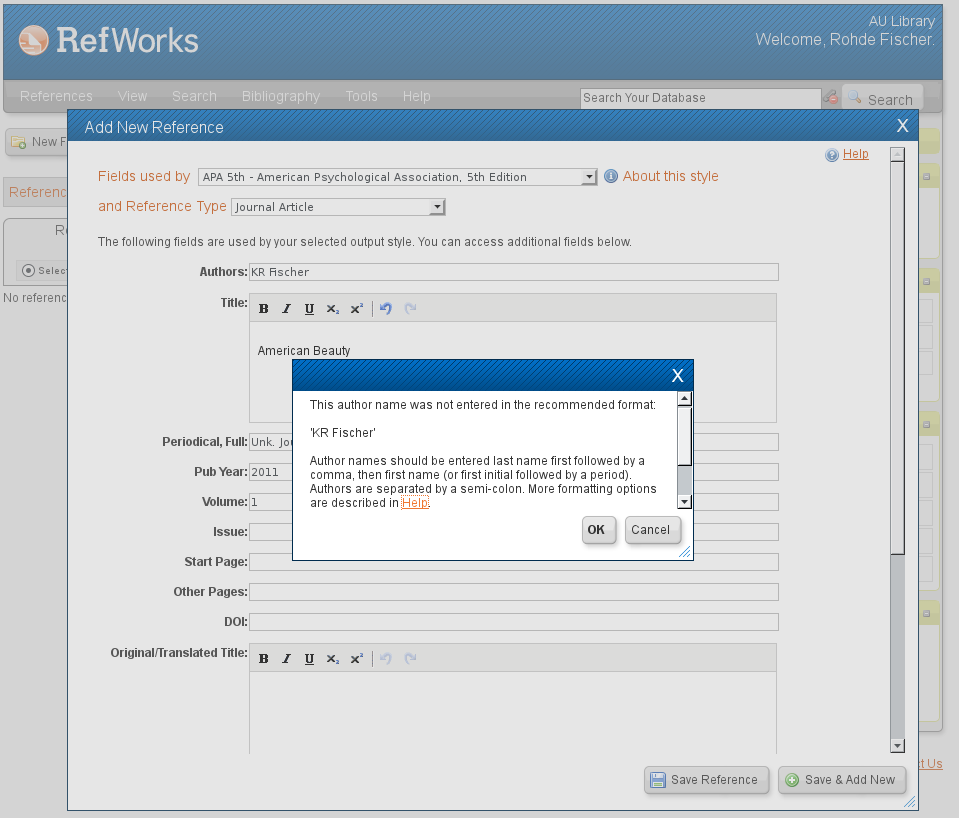
\includegraphics[width=0.8\textwidth]{refworks-detect-formatting}
    \caption{RefWorks detects some formatting on the name field}
    \label{fig:refworks-detect-formatting}
\end{figure}

In RefWorks itself there seems to be no spell checker, but this is in
part solved by most modern browsers, because they tend to include
spell checkers for input fields.

\subsection{Zotero}
Zotero is a reference manager developed by Roy Rosenzweig Center for
History and New Media.  It is targeted at people doing research.  The
organization and collaboration aspects are in focus for
Zotero\cite{zotero_features}.

There is a built in spell checker for notes written in Zotero, however
the spell checker is not applied for things like titles, which
prevents it from detecting those errors.  Like JabRef, Zotero has a
plugin system, on found using the official list of plugins
\cite{zotero_plugins} nor by a normal search engine. There is a
limited mechanism for detecting abbreviations in Zotero, in its
jar-file there is a list of known abbreviations which it can use to
chose the correct abbreviation when exporting, entering a known
abbreviation does not seem to correct it to the non-abbreviated
version.  This list can be manually edited, and overruled
\cite{zotero_abbreviations}.

It is possible (but not tested) that Zotero can be used to import an
Bib{\TeX}-file, then export it using the lists of known abbreviations
and correct the abbreviations already known.  As other tools such as
JabRef and Mendeley will already allow this, it has not been tested.

\subsection{Papers}
Papers is a reference manager developed by Mekentosj B.V., targeted
for science and research.  It provides a tool set for searching online
libraries for references, collaboration and various ways of
organizing \cite{papers_features}.

It does not highlight any features of relevance \cite{papers_features}
and as it is developed for Mac OS, it has not been possible to test if
there is relevant features apart from what they mention on their page.

\section{Research \remark{better headline name would be ideal}}
It has not been possible to find research covering the issues of
interest, such as inconsistencies and spelling errors, in Bib{\TeX}
documents.  The issues has been partially handled on the practical
level, which can be seen in sections \ref{sec:bibtex_tools} and
\ref{sec:bib_managers}.  However issues such how to disambiguate
abbreviations has been a concern in others contexts.

\subsection{Abbreviation disambiguation using Machine Learning}
In \cite{okazaki2010_building} machine learning is used to classify
abbreviations to allow disambiguation.  The method they used has the
expanded forms and the abbreviations, since there may be multiple
expanded forms concerning the same abbreviation (eg. ``polymerase
chain reaction `` and ``polymerization chain reaction``), they
introduce a sense inventory which is a cluster for things having the
same meaning.

The technique is quite powerful and has

\subsection{ALICE}
ALICE is an abbreviation detection system for bio articles. It uses a
lot of rules to detect abbreviation styles.

Perhaps some of those rules can be reused in my project?

\subsection{Overview}
\remark{I know, needs work}

Abbreviation detection in Bib{\TeX} will usually only have one
expanded form for each use of an abbreviation.  There may be a journal
named FooBar and one named FooBaz, both using the abbreviation FB,
however if FB is expanded to FooBar it will not occur that it is in
the sense of FooBar's or other variations, since the journal name is
just the name and not in a textual context where variations will
occur.  Thus a clustering based system like in
\cite{okazaki2010_building} will be overkill.  It is possible that a
machine learning approach will acchieve more accuracy, but the
approach has been put aside in this dissertation for simplicity.

%The work in \cite{?} has a more practical approach as it uses simple
%rules for when something can be considered an abbreviation.  However
%they make the assumption that the expansion of an abbreviation will be
%located close to it at one of its uses.  However in Bib{\TeX} it is
%likely that it is either located elsewhere in the file or not in the
%file at all.

%%% Local Variables:
%%% mode: latex
%%% TeX-master: "thesis"
%%% End:
